\section{Ontology-Based Activity Modelling}
\label{sec:approach:ontology}

Ontology-based activity modelling has already been introduced in Chapter \ref{cha:soa}, concretely in Section \ref{subsec:soa:ontology}. Some of the most relevant research works were presented there. However, the objective of this section is to provide a deep description of one of the presented approaches, which is the basis of the contributions presented in this dissertation.

The activity modelling approach introduced in \cite{Chen2012a} is central to the real-time activity recognition system for smart homes described in the paper. This approach has been designed for the dense sensing-based activity monitoring scenario and deployed in a smart home research laboratory, obtaining an average activity recognition rate of 94.44\%. The reported results suggest that the system performs robustly for selected scenarios.

Even though the activity recognition process is very interesting, the focus of this section will be on the ontology-based activity modelling approach which is introduced in \cite{Chen2012a}. Roughly speaking, two high-level concepts are modelled in the paper to support activity recognition: (i) Activities of Daily Living (ADL) and (ii) the context in which those ADLs are performed (in the case of the paper, a smart home). To specify conceptual structures and relationships, DL based markup language, i.e. Web Ontology Language (OWL) and Resource Description Framework (RDF)\footnote{http://www.w3.org/} are used. Both languages support inference and reasoning, a feature which plays a key role for activity recognition. 

\subsection{Ontological ADL Modelling}
Activities of Daily Living, or ADLs, refer to a set of activities that are performed by any person in a daily basis. Some examples for ADLs are making tea, making pasta or washing dishes. When ADLs are carefully analysed, two features can be identified: (i) ADLs can be defined at different levels of granularity, and (ii) ADLs are generic, but each person perform them in different ways. Both features can be properly addressed by the ontological ADL modelling approach.

The first feature, activity granularity, refers to the fact that ADLs form super-class and sub-class relations. For example, making a hot chocolate can be considered a sub-activity of making a hot drink, which can also be classified as a sub-activity of making a drink. As such, ADLs form a tree where leafs model \textit{primitive} ADLs and other nodes refer to \textit{composite} ADLs (see Figure \ref{fig-adl-granularity}).

\begin{figure}[htbp]%[!t]
\centering
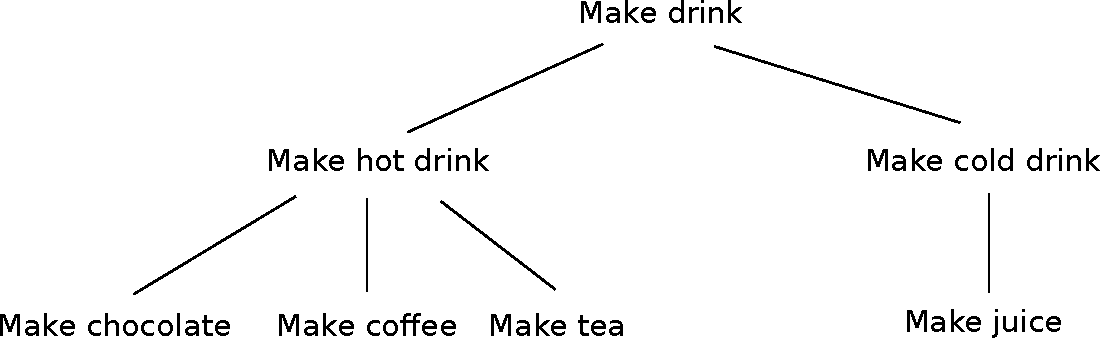
\includegraphics[width=\textwidth]{ADL_granularity.pdf}
    \caption{An example of ADL granularity represented as a tree.} 
    \label{fig-adl-granularity}
\end{figure}

To address different levels of activity granularity, ontological modelling, i.e. the process to explicitly specify key concepts and their properties for a problem domain, is applied. More concretely, ADLs are modelled as ontological concepts which are organised in a hierarchical structure in terms of their shared properties to form super-class and sub-class relations. Those relations between primitive and composite ADLs are characterised by ``is-a'' and ``part-of'' relationships, properly supported by OWL. For example, as shown in Figure \ref{fig-adl-granularity} making tea is a subclass of making hot drink. The ADL for making tea is represented by the ontological concept of MakeTea, while making hot drink is represented by MakeHotDrink. Properties establish the interrelations between concepts. For instance, \textit{hasDrinkType} is a property of the MakeHotDrink activity that links the DrinkType concept (e.g., tea, coffee, chocolate) to the MakeHotDrink concept. Both, concepts and properties, are modelled using the commonly shared terms in the problem community. The resulting ontologies are essentially knowledge models able to encode and represent domain knowledge and heuristics. 

The second feature highlights the difference between generic and personalised ADLs. Even though making coffee implies the use of coffee and a container, some users prefer African coffee to Colombian coffee and some users use cups and others mugs. Furthermore, the order of the sequence of objects used to making coffee, vary from user to user, e.g. some users might add sugar before coffee and others add sugar once coffee has been poured to the container. In consequence, generic and personalised ADLs can be distinguished.

\begin{enumerate}
 \item Generic activity models: defined at the conceptual level as an activity class described by a number of properties. These properties describe the types of objects and their usage to perform an activity. Generic activity models are applicable to all users.
 \item Personalised activity models: they capture the specific way of a user to perform an activity and are modelled as instances of a corresponding conceptual activity model, which consists of specific information related to the concrete objects used and the sequential order they are used in.
\end{enumerate}

Activities are defined as ontological concepts and all actions that are required to perform the activity as the properties of the concept. For example, making tea involves taking a cup from the cupboard, putting a teabag into the cup, adding hot water to the cup, then milk and/or sugar. The ontological model of making tea, i.e. MakeTea concept, can be defined by action properties \textit{hasContainer}, \textit{hasTeabag}, \textit{hasHotwater}, \textit{hasMilk} and \textit{hasFlavour} in conjunction with descriptive properties such as activity start time \textit{actStartTime} and duration \textit{actDuration}. Notice that two kinds of properties are defined: \textit{action properties}, which refer to action-based properties and \textit{descriptive properties}, which are used to characterise the manner in which an activity is performed. This distinction is very important, because action properties play a crucial role for activity recognition. Indeed, activities are inferred from action properties which are generated by the sensor activations occurring due to human-object interactions. On the other hand, descriptive properties are not determinant in activity recognition. For instance, making coffee can happen at any time, it can be performed in different sequences and it may take variable amounts of time. As such, descriptive properties are used to model user's activity profiles, which are not used for the activity recognition process.

Hence, action properties define generic ADL models, which are used for activity recognition and are applicable to any user. Descriptive properties capture the different ways of performing generic ADLs, in terms of the objects used, the order in which those objects have been used, activity start time and duration. Personalised ADL models are instances of the corresponding generic ADL model.

In summary, ontological ADL modelling properly addresses different levels of activity granularity and the difference between generic and personalised ADLs, using the tools provided by markup languages such as OWL and RDF. 

\subsection{Ontological Context Modelling}

The ADL modelling scheme described above establishes a clear dependency between the context and an ADL. Indeed, ADLs are described as a set of context events, where context refers to temporal, spatial, event and environmental aspects. Example temporal aspects of an ADL may be the start time and the duration of the activity, which are captured by descriptive properties. Spatial aspects relate to location information and surrounding entities such as rooms, household furniture and appliances. Event contexts capture dynamic state changes of the objects of the environment, for example, state changes of doors, fridge door or a microwave oven. Those events are modelled by action properties. Finally, environmental aspects of the context are composed of environmental information such as temperature, humidity and general weather conditions. 

In the dense sensing paradigm, contextual information is captured through various sensors. Each sensor monitors and reflects one facet of a situation. Based on this observation the context modelling is centred on ontological sensor modelling. Sensors are inherently linked to a number of physical and conceptual entities such as objects, locations and states. For example, a contact sensor is attached to a teapot in the second cupboard to the left of the sink in the kitchen. By explicitly capturing and encoding such domain knowledge in a sensor model it is possible to infer the corresponding objects and location from the activation of the sensor. This implies that an inhabitant performs an activity in the inferred location with the inferred object.

As most ADLs require the interlinking and fusion of data from multiple, disparate sensor sources in order to infer the high-level activities, it is necessary to aggregate a sequence of sensor activations to generate a situation at a specific time point. The situation formation process can be described as follows. Each sensor has a default state value for its state property, denoting the state of the object to which it is attached. When a sensor is activated, the state property will change. Subsequently the system will translate the state change as an occurrence of a user- object interaction at the specific time. As it is difficult, if not impossible, to monitor what happens at detailed levels after an object is interacted with, it is common practice to interpret a sensor activation as a user-object interaction, ignoring how the object is used and when it is de-activated. As such a user-object interaction is equivalent to an instantaneous sensor activation and can be interpreted as an object has been used for performing an activity. In this way, by aggregating individual user-object interactions along a timeline the situation at specific time points can be generated. 

Under this context modelling approach, sensor activations are assumed to be produced by user-object interactions, which may denote an action property or a descriptive property, depending on the nature of the object and sensor. For example, a thermometer state change will be captured by a descriptive property such as \textit{hasTemperature(value)}, whereas a contact sensor installed in a cup will generate the action property \textit{hasContainer(cup)}. 

\subsection{Final Remarks about Ontology-Based Activity Modelling}

A common framework to model ADLs and contextual information is provided by the ontology-based activity modelling approach described in \cite{Chen2012a}. Ontology-based activity modelling provides semantically clear, structured and reusable models. Furthermore, it offers a unified framework to combine generic models that can be applied to any user with personal models. By means of ontological modelling some traditional problems of data-driven approaches can be avoided, such as the manual class labelling, pre-processing and training processes. In addition, ontologies allow software agents to interpret data and reason against ontological contexts, thus enhancing the capabilities of automated data interpretation and inference.

However, the main problem of this modelling approach is related to model incompleteness. Obtaining complete models from domain knowledge for every person is not generally possible. An ADL model is composed by action and descriptive properties, so model incompleteness refers to the impossibility of completely define all the action and descriptive properties of an ADL. In the case of descriptive properties, model incompleteness is obvious, since those properties refer to personalised ways of performing activities. Chen et al. propose in \cite{Chen2014} a hybrid activity modelling approach to learn descriptive properties from user generated data. But they consider that ADL models in terms of action properties are complete. This assumption does not generally hold, because even though there are certain actions that every user performs for a given activity, there might be some other actions that cannot be known in the modelling step. 

Hence, this dissertation tackles the problem of learning unmodelled action properties for activity models. By means of learning new actions through incremental data-driven learning techniques, the static and generic nature of knowledge-driven activity models is also tackled. The contributions of this dissertation allow dynamic activity models which evolve in time and support both, generic and personalised models.